\documentclass[11pt]{article}

\usepackage[utf8]{inputenc}
\usepackage[T1]{fontenc}
\usepackage[french]{babel}
\usepackage[top=1.8cm, bottom=1.8cm, left=1.8cm, right=1.8cm]{geometry}
\usepackage{hyperref}
\usepackage{graphicx}
\usepackage{epsfig}
\usepackage{amssymb}
\usepackage{amsmath}
\usepackage{array}
\usepackage{subfig}
\usepackage{multicol}
\usepackage{caption}
\usepackage{algorithm}
\usepackage{algorithmic}
\hypersetup{
    colorlinks=true,
    breaklinks=true,
    urlcolor=red,
}
\parskip=5pt

\title{\huge{\textbf Cahier des charges}}
\author{AYOUB Pierre, BASKEVITCH Claire, BESSAC Tristan, \\
CAUMES Clément, DELAUNAY Damien, DOUDOUH Yassin}
\date{Mercredi 14 Mars 2018}

\begin{document}

\maketitle
\vspace{20em}
\begin{center}
\includegraphics{pictures/Application.png}\end{center}

\small
\section{Préambule}

\subsection{Définition des termes du sujet}

La stéganographie est l'art de la dissimulation, appliquée en informatique en
cachant des données dans d'autres données. Cette dissimulation se fait
généralement au sein de fichiers multimédias. La stéganographie se différencie
de la cryptographie, qui correspond à chiffrer un message afin qu'il soit
illisible par une personne différente de l'émetteur et du destinataire. En
effet, un message chiffré en cryptographie sera visible par tous mais illisible,
tandis qu'un message caché dans un fichier $f$ en stéganographie ne sera vu que
si un inconnu sait que $f$ contient un message et connaît l'algorithme pour
l'interpréter. 

La stéganalyse, quant à elle, est la recherche de données cachées dans des
fichiers suspects. Si ces données sont identifiées, il faut ensuite réussir à
les extraire pour les lire. Il s'agit donc de la méthode inverse à la
stéganographie. 

\subsection{Historique}

La stéganographie est une méthode très ancienne dont la première référence à
cette utilisation date du premier siècle avant Jésus-Christ. Elle apparaît dans
un récit écrit par Hérodote qui raconte comment deux citoyens communiquaient
secrètement : le premier citoyen rasait la tête de son esclave et lui écrivait
un message sur son crâne. Ensuite, il fallait attendre que les cheveux de
l'esclave repoussent puis envoyer ce dernier chez le deuxième citoyen. Ce
citoyen devait de nouveau raser la tête de l'esclave pour découvrir le message
qui lui était destiné. Une autre utilisation de la stéganographie consistait à
utiliser de l'encre, invisible à l'oeil nu, mais qui était révélée à la chaleur.

Avec l'émergence de l'informatique, les techniques de stéganographie se sont
renouvelées. En effet, il est désormais possible de cacher des données dans
d'autres données. Cette multiplicité de techniques stéganographiques, grâce à
l'informatique, montre l'étendue de cette application dans tous les domaines.
Par exemple, la stéganographie moderne a été utilisée dans des communications
terroristes (transmission de messages) ou dans les signatures de fichiers
multimedia (tatouage numérique) afin de protéger les droits d'auteurs. 

\section{Conducteurs du projet}

\subsection{But du projet}

Le but du projet est de réaliser un logiciel de stéganographie permettant à des
personnes lambdas de communiquer sans que l'on soupçonne que leurs
communications soient en réalité compromettantes. Le but de l'application est
de permettre à un utilisateur $U_1$ d'envoyer des données cachées à un autre
utilisateur $U_2$. Ce deuxième utilisateur devra pouvoir interpréter ces données
en utilisant la même application que $U_1$. 

\subsection{Motivation du projet}

La motivation du projet est venue par notre envie de la majorité des membres de
ce groupe de projet d'obtenir le master SeCReTs. En effet, nous voulions tous
réaliser un projet en rapport à la cryptographie et c'est donc pour cela que
nous nous sommes réunis afin de réaliser ce type de projet. 

\section{Contraintes du projet}

\subsection{Calendrier}

Le calendrier est imposé et suit les étapes suivantes : 

\begin{itemize}
\item Le cahier des charges doit être remis le 14 mars.
\item Le cahier des spécifications est à remettre le 18 avril.
\item La remise du produit au client est le 25 mai.
\item La présentation du produit au client sera le 1 juin.
\end{itemize}


\subsection{Contraintes imposées}

Plusieurs contraintes sont imposées par le client : 

\begin{itemize}
\item Le produit permettra à celui qui l'utilise de cacher des données dans des
    fichiers de différents types : les images, le son et la vidéo seront pris
    en charge. Les formats seront choisis par le concepteurs de
    l'application. 
\item Le fichier à analyser est le fchier hôte : on sait à l'avance que celui-ci
    contient des données à extraire et il faut donc les prélever. 
\item L'application aura une interface graphique : elle sera manipulée par les
    utilisateurs voulant découvrir un message envoyé par quelqu'un ayant
    utilisé cette même application, ou voulant cacher des données dans un
    fichier. Il devra néanmoins choisir un fichier hôte que l'application
    puisse manipuler. 
\item Le logiciel proposera également une interface en ligne de commande, qui
    proposera les mêmes fonctionnalités que l'interface graphique. 
\end{itemize}

\section{Exigences fonctionnelles}

\subsection{Portée du produit}

L'application sera utilisée par des utilisateurs qui pourront tous faire les
mêmes actions. La première consiste en la dissimulation des données dans un
fichier, tandis que la seconde consiste en l'extraction des données cachées
depuis le fichier hôte. Cela permettra à un utilisateur d'insérer des données à
cacher dans un fichier, afin de l'envoyer à un autre utilisateur. Ce dernier va
ensuite faire la tâche inverse pour les récupérer.

\subsection{Exigences du client}

L'application doit respecter deux exigences pour le client : elle doit permettre
à un utilisateur ne connaissant pas la stéganographie de pouvoir facilement
utiliser toutes les fonctionnalités de l'application grâce à une interface
graphique intuitive. De plus, une interface en ligne de commande doit être
également proposée pour les utilisateurs sachant manipuler un programme dans un
terminal. 
%Cela permettra à ces utilisateurs plus expérimentés d'intégrer
%l'application dans des scripts.

\section{Exigences non fonctionnelles}

\subsection{Apparence et perception}

Le logiciel doit permettre à n'importe quel utilisateur de pouvoir cacher ses
données dans des fichiers. En effet, la facilité d'utilisation de l'application
sera ciblée pour le développement. Il sera facile de naviguer entre les deux
menus en fonction de si l'utilisateur veut cacher ses données ou s'il veut
extraire les données cachées d'un fichier. Il pourra naviguer dans son système
de gestion de fichiers afin de choisir le fichier hôte et quel fichier
contiendra ces données cachées. 

\subsection{Performance}

L'application devra être rapide pour l'utilisateur qui s'en sert. Bien entendu,
la stéganographie sur certains fichiers lourds (tels que des fichiers vidéos)
rendra l'exécution plus lente mais elle ne devra pas être trop importante pour
l'utilisateur. 

\subsection{Exigences culturelles, politiques et légales}

L'application de stéganographie vise des clients en France. Il faut donc
respecter les lois françaises concernant l'utilisation de cette application. La
loi du 21 juin 2004, pour la confiance dans l'économie numérique, définit cette
application comme moyen de cryptologie car elle vise à transformer des données
pour garantir la sécurité de la transmission de celles-ci. Par ailleurs,
l'article 30 de cette même loi oblige la déclaration de l'application si cette
dernière est importée et/ou exportée. 

\section{Modules du produit}

\subsection{Organigramme}

\hspace{1cm}
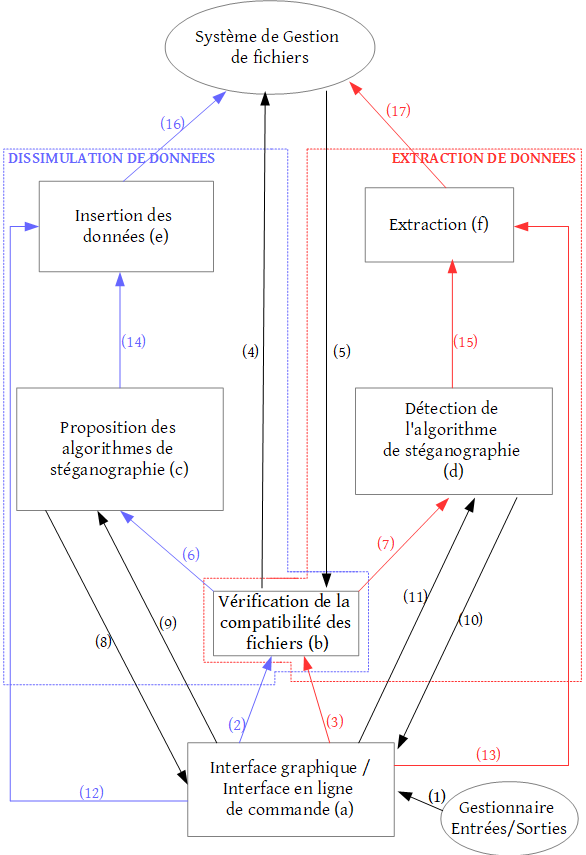
\includegraphics[scale=0.71]{pictures/organigramme.png}

\paragraph{Liste des modules et de leurs fonctionnalités :}

\begin{description}
\small
\item[a)] \textbf{Interface graphique / Interface en ligne de commande} :
    interfaces permettant à l'utilisateur de choisir parmi les deux
    fonctionnalités possibles de l'application. Il peut dissimuler des
    données dans un fichier (dont le type et le format sont pris en charge
    par l'application). Ou bien, il peut extraire les données cachées d'un
    fichier. \newline
    Il aura donc un mécanisme pour choisir le fichier hôte et le fichier 
    à cacher (pour la dissimulation de données), et un mécanisme pour choisir le 
    fichier contenant les données cachées à analyser (pour l'extraction de 
    données cachées). 
    

\item[b)] \textbf{Vérification de la compatibilité des fichiers} : le format 
	du fichier hôte (pour le module \textit{Dissimulation de données}) ou 
	le format du fichier à analyser (pour le module \textit{Extraction de données 
	cachées}), choisis par l'utilisateur, est vérifié pour savoir s'il est 
	bien pris en charge par l'application. \newline
	Il aura un mécanisme de lecture du fichier hôte (pour la dissimulation 
	des données) : selon les formats pris en charge, il y aura une batterie
	de tests pour déterminer le format du fichier. 

\item[c)] \textbf{Proposition des algorithmes de stéganographie} : en fonction
    du type et du format du fichier hôte, ainsi que de la taille des données à
    cacher, un mécanisme proposera un ou plusieurs algorithmes. 

\item[d)] \textbf{Détection de l'algorithme de stéganographie} : un mécanisme 
	d'analyse du fichier permettra de découvrir quel algorithme a été utilisé 
	afin de les extraire correctement par la suite. 

\item[e)] \textbf{Insertion des données} : la copie des données du fichier hôte
    sera modifiée avec l'insertion des données à cacher à l'aide de l'algorithme
    choisi par l'utilisateur. 

\item[f)] \textbf{Extraction} : les données cachées dans le fichier à analyser
    sont extraites. Les algorithmes utilisés pour l'insertion des données 
    et l'extraction seront expliqués dans la sous-section \textit{"Algorithmes 
    de dissimulation et d'extraction en stéganographie"}

\end{description}

\paragraph{Liste des informations qui circulent entre les modules :}

\begin{multicols}{2}
\begin{description}
\small
\item[1)] 
\begin{itemize}
\item Utilisation de l'application (dissimulation ou extraction).
\item Nom du fichier hôte, nom du fichier à cacher et chemin du fichier à créer
    (pour la dissimulation).
\item Nom du fichier à analyser et chemin du fichier résultant de l'extraction
    des données cachées (pour l'extraction).
\end{itemize}
\item[2)] 
\begin{itemize}
\item Nom du fichier hôte.
\item Nom du fichier à cacher.
%\item Chemin du fichier à créer qui dissimulera les données à cacher et aura
    %l'apparence du fichier hôte.
\end{itemize}
\item[3)] 
\begin{itemize}
\item Nom du fichier contenant les données cachées à analyser.
%\item Chemin du fichier résultant de l'extraction des données cachées.
\end{itemize}
\item[4)] 
\begin{itemize}
\item Nom du fichier hôte et nom du fichier à cacher (pour la dissimulation).
\item Nom du fichier contenant les données cachées à analyser (pour
    l'extraction).
\end{itemize}
\item[5)]
\begin{itemize}
\item Fichier hôte et fichier à cacher (pour la dissimulation).
\item Fichier contenant les données cachées à analyser (pour l'extraction).
\end{itemize}
\item[6)]
\begin{itemize}
\item Fichier hôte.
\item Fichier à cacher.
%\item Chemin du fichier à créer qui dissimulera les données à cacher.
\end{itemize}
\item[7)]
\begin{itemize}
\item Fichier contenant les données cachées à analyser.
%\item Chemin du fichier résultant de l'extraction des données cachées.
\end{itemize}
\item[8)]
\begin{itemize}
\item Liste des algorithmes que l'utilisateur peut utiliser (selon le format du
    fichier hôte et la taille des données à cacher).
\end{itemize}
\item[9)]
\begin{itemize}
\item Choix de l'algorithme par l'utilisateur.
\item Mot de passe choisi par l'utilisateur (s'il a choisi l'option de protéger
    ses données par mot de passe).
\end{itemize}
\item[10)]
\begin{itemize}
\item Choix de l'algorithme détecté dans le fichier à analyser.
\end{itemize}
\item[11)]
\begin{itemize}
\item Mot de passe pour extraire les données (s'il a choisi l'option de
    protéger ses données par mot de passe).
\end{itemize}
\item[12)]
\begin{itemize}
\item Chemin du fichier à créer qui dissimulera les données à cacher et aura
    l'apparence du fichier hôte.
\end{itemize}
\item[13)]
\begin{itemize}
\item Chemin du fichier résultant de l'extraction des données cachées.
\end{itemize}
\item[14)]
\begin{itemize}
\item Fichier hôte.
\item Fichier à cacher.
%\item Chemin du fichier à créer lors de la dissimulation de données.
\item Nom de l'algorithme de stéganographie utilisé.
\item Mot de passe choisi par l'utilisateur (s'il a choisi l'option de protéger
    ses données précédemment).
\end{itemize}
\item[15)]
\begin{itemize}
\item Fichier contenant les données cachées à analyser.
%\item Chemin du fichier résultant de l'extraction des données cachées.
\item Nom de l'algorithme détecté.
\item Mot de passe choisi par l'utilisateur (s'il a choisi l'option de protéger
    ses données précédemment).
\end{itemize}
\item[16)]
\begin{itemize}
\item Données de l'hôte où les données à cacher ont été insérées en utilisant
    l'algorithme de stéganographie.
\end{itemize}
\item[17)]
\begin{itemize}
\item Données cachées extraites du fichier hôte.
\end{itemize}
\end{description}
  \ldots
\end{multicols}

%\normalsize
\small
\subsection{Algorithmes de dissimulation et d'extraction en stéganographie}

L'application permettra de cacher des données dans des fichiers de différents
types (image, son, video). Pour le calcul de complexités, nous avons utilisé les symboles suivants : 
$n$ pour la taille en octets du fichier caché (ou à cacher) et $m$ pour la taille 
en octets du fichier hôte ne contenant pas les données cachées. 

\subsubsection{Algorithme LSB (Least Significant Bit)}

L'algorithme LSB permet de cacher des bits dans des octets tel qu'ils seront
invisibles pour l'Homme. Il permet de cacher des données dans un fichier sans en
altérer sa taille. Dans le cas de la stéganographie sur une image non compressée,
chaque pixel d'une image correspond à un triplet de nombres dit triplet RGB. Ce
triplet correspond aux composantes de couleurs Rouge-Vert-Bleu, prenant des
valeurs allant de 0 à 255. Le but de cet algorithme est donc de cacher des bits 
dans cette image. Pour se faire, nous allons remplacer les 2 bits de poids 
faibles de chaque composante des pixels de l'image. En effet, à l'oeil nu, 
l'homme ne discernera jamais le changement minime de couleur induis par la 
modification. 

\begin{minipage}{.5\textwidth}
\begin{algorithm}[H]
\caption{Dissimulation Algorithme LSB}
\begin{algorithmic}
\color{green}
\STATE \footnotesize Entrées : fichier à cacher, fichier hôte
\color{black}
\STATE  Ouverture fichier à cacher (LECTURE) $\rightarrow$ $f1$
\STATE Ouverture fichier hôte (LECTURE) $\rightarrow$ $f2$
\STATE Ouverture fichier final (ECRITURE) $\rightarrow$ $f3$
\WHILE{(Fin de fichier $f1$ non atteinte)}
\STATE $b1 = $LECTURE 2 bits ($f1$)
\STATE $o1 = $LECTURE octet ($f2$)
\STATE $o1 = $CHANGEMENT\_BIT\_POIDS\_FAIBLE($o1$,$b1$)
\STATE ECRITURE $o1$ dans $f3$
\ENDWHILE
\WHILE{(Fin de fichier $f2$ non atteinte)}
\STATE $o1 =$LECTURE octet ($f2$)
\STATE ECRITURE $o1$ dans $f3$
\ENDWHILE
%\STATE ECRITURE suite d'octets ($f3$) $\rightarrow$ identification algo, nom fichier caché, taille données cachées
\STATE Fermeture fichiers $f1$, $f2$, $f3$
\color{green}
\STATE Sortie : fichier final
\color{black}
\end{algorithmic}
\end{algorithm}
\normalsize
\end{minipage}
\begin{minipage}{.5\textwidth}
\begin{algorithm}[H]
\caption{Extraction Algorithme LSB}
\begin{algorithmic}
\color{green}
\STATE \footnotesize Entrée : fichier à analyser
\color{black}
\STATE Ouverture fichier à analyser (LECTURE) $\rightarrow$ $f1$
\STATE Ouverture fichier extrait (ECRITURE) $\rightarrow$ $f2$
\STATE Taille $\leftarrow$ 0
\WHILE{(Taille < [taille bits fichier caché])}
\STATE $o1 = $LECTURE octet (f1)
\STATE $b1 = $2\_BITS\_POIDS\_FAIBLE($o1$)
\STATE ECRITURE $b1$ ($f2$)
\STATE Taille = Taille + 2
\ENDWHILE
\STATE Fermeture $f1$, $f2$
\color{green}
\STATE Sortie : fichier extrait
\color{black}
\end{algorithmic}
\end{algorithm}
\normalsize
\end{minipage}

%Prenons un exemple de couleur
%$C_1$ dont le triplet est $(219,27,91)$. 

%R : $219_{10} = 11011011_2$ \qquad G : $27_{10} = 00011011_2$
%\qquad B : $91_{10} = 01011011_2$

%Imaginons que la donnée à cacher dans le fichier composé de cet unique pixel de
%couleur $C_1$ correspond à la suite de bits $B = 000000_2$. Après modification
%des 2 bits de poids faibles de chaque composants du pixel, cela donne une
%autre couleur $C_2$ défini par le triplet suivant : 

%R : $216_{10} = 11011000_2$ \qquad G : $24_{10} = 00011000_2$
%\qquad B : $88_{10} = 01011000_2$

%La figure suivantes illustres les deux couleurs $C_1$ et $C_2$ côte à côte,
%montrant ainsi qu'un humain ne pourra jamais détecter un changement de bit : 

%\begin{figure}[h]
% \begin{minipage}{.46\linewidth}
%  \centering\epsfig{figure=pictures/219_27_91.png}
%  \caption{Couleur $C_1$}
% \end{minipage} \hfill
% \begin{minipage}{.46\linewidth}
%  \centering\epsfig{figure=pictures/216_24_88.png}
%  \caption{Couleur $C_2$}
% \end{minipage}
%\end{figure}

La complexité de la dissimulation se calcule de la manière suivante : 
la première boucle TantQue a une complexité de $O(m-n)$, la deuxième $O(n)$. 
\newline Donc la complexité de la dissimulation LSB est de $O(m-n)+O(n)=O(m-n+n)=O(m)$, 
puisqu'on intégre directement les données cachées dans les données de l'hôte. 
\newline La complexité de l'extraction LSB est, quant à elle, de $O(n)$.

Cet algorithme peut également s'appliquer à d'autres types de fichiers. Pour le
son non compressé, il est possible de très peu modifier l'amplitude de chaque
échantillon de son, de telle manière que l'on peut y cacher des données sans
altérer le son original pour la perception humaine. Pour la vidéo non compressé,
un tel fichier est composé d'un enchaînement de multiples frames (images) et il
est donc possible de manipuler les données pour pouvoir en cacher d'autres, de
la même manière que pour les deux autres types de fichier cités précédemment.

%Pour la partie réception du fichier, il faut connaître combien de bits sont
%cachés. Il faudra donc calculer la taille maximale du message à cacher qui sera
%une puissance de 2. En effet, en fonction de la taille du fichier, un certain
%nombre de bits sera réservé pour connaître la taille des données à cacher. En
%fonction de ces informations, la suite de bits cachée sera donc formée.

\subsubsection{Algorithme EOF (End Of File)}

Chaque format de fichier a une mise en forme unique permettant de décrire le
type de données souhaité. L'entête du fichier va contenir la signature du
format, appelé le Magic Number, ainsi que plusieurs autres octets décrivant ce
fichier. Le reste du fichier contient le contenu visible par l'utilisateur grâce
à l'application appropriée. 

Pour que l'application utilisée par l'utilisateur sache quand la lecture du
fichier doit s'arrêter, certains formats de fichier continnent, à la toute fin,
un octet représentant la fin du fichier (EOF). Si des données existent après ce
EOF, elles ne seront pas interprétées par l'application. L'algorithme EOF est un
algorithme très utilisé dans la stéganographie pour cacher des données : il
consiste à écrire une suite de bits représentant les données à cacher
directement à la fin du fichier hôte.
En revanche, cet algorithme souffre de plusieurs faiblesses, notamment 
le fait que la taille du fichier hôte se voit incrémenté de la taille 
des données à cacher.

\begin{minipage}{.5\textwidth}
\begin{algorithm}[H]
\caption{Dissimulation Algorithme EOF}
\begin{algorithmic}
\color{green}
\STATE \footnotesize Entrées : fichier à cacher, fichier hôte
\color{black}
\STATE Ouverture fichier à cacher (LECTURE) $\rightarrow$ $f1$
\STATE Ouverture fichier hôte (LECTURE) $\rightarrow$ $f2$
\STATE Ouverture fichier final (ECRITURE) $\rightarrow$ $f3$
\WHILE{(Fin de fichier $f2$ non atteinte)}
\STATE $o1 = $LECTURE octet ($f2$)
\STATE ECRITURE $o1$ ($f3$)
\ENDWHILE
\WHILE{(Fin de fichier $f1$ non atteinte)}
\STATE $o1 =$LECTURE octet ($f1$)
\STATE ECRITURE $o1$ dans $f3$
\ENDWHILE
\STATE Fermeture fichiers $f1$, $f2$, $f3$
\color{green}
\STATE Sortie : fichier final
\color{black}
\end{algorithmic}
\end{algorithm}
\normalsize
\end{minipage}
\begin{minipage}{.5\textwidth}
\begin{algorithm}[H]
\caption{Extraction Algorithme EOF}
\begin{algorithmic}
\color{green}
\STATE \footnotesize Entrée : fichier à analyser
\color{black}
\STATE Ouverture fichier à analyser (LECTURE) $\rightarrow$ $f1$
\STATE Ouverture fichier extrait (ECRITURE) $\rightarrow$ $f2$
\STATE Taille $\leftarrow$ 0
\STATE Placement curseur EOF "officiel" fichier à analyser
\WHILE{(Taille < [taille octets fichier caché])}
\STATE $o1 = $LECTURE octet (f1)
\STATE ECRITURE $o1$ ($f2$)
\STATE Taille = Taille + 1
\ENDWHILE
\STATE Fermeture $f1$, $f2$
\color{green}
\STATE Sortie : fichier extrait
\color{black}
\end{algorithmic}
\end{algorithm}
\normalsize
\end{minipage}

Pour la dissimulation EOF, la première boucle TantQue a une complexité de $O(m)$, 
la deuxième $O(n)$. \newline Donc sa complexité globale pour l'algorithme 
EOF est de $O(m)+O(n)=O(m+n)$. \newline
La complexité de l'extraction EOF dépend seulement de la taille du fichier 
caché, soit $O(n)$.

\subsubsection{Méthode manipulant les métadonnées}

Les fichiers multimédias, tels que les images, les sons et les vidéos,
contiennent plusieurs types de données. Tout d'abord, la majeure partie du
fichier représente les données du fichier en elles-mêmes. Dans le cas d'une
image, on pourrait donner l'exemple des données représentant chaque pixel de
l'image. 

Mais souvent, en amont des données principales du fichier, il existe les
métadonnées servant à décrire le fichier représenté. Par exemple, il y a 
aussi des zones du fichier réservées à l'utilisateur afin qu'il y mette des 
 "commentaires", par exemple pour représenter l'origine du fichier ou 
encore des informations sur la prise de vue dans le cas d'une photo. 
Les métadonnées sont affichés si l'utilisateur le demande, mais sont en 
général cachés par défaut.

De ce fait, les métadonnées sont très utilisées en stéganographie. Elles
permettent d'insérer des données qui seront à premère vue invisible pour
l'utilisateur. Pour pouvoir cacher des données en manipulant les métadonnées,
il faut donc analyser chaque format pris en charge par l'application afin de
connaître les détails des différents morceaux de données présents dans le
fichier. 

\begin{minipage}{.5\textwidth}
\begin{algorithm}[H]
\caption{Dissimulation Algorithme MetaData}
\begin{algorithmic}
\color{green}
\STATE \footnotesize Entrées : fichier à cacher, fichier hôte
\color{black}
\STATE Ouverture fichier à cacher (LECTURE) $\rightarrow$ $f1$
\STATE Ouverture fichier hôte (LECTURE) $\rightarrow$ $f2$
\STATE Ouverture fichier final (ECRITURE) $\rightarrow$ $f3$
\WHILE{(Fin de fichier $f2$ non atteinte)}
\STATE $o1 = $LECTURE octet ($f2$)
\STATE ECRITURE $o1$ ($f3$)
\IF{($o1 ==$ curseur où insérer MetaData)}
\WHILE{(Fin de fichier $f1$ non atteinte)}
\STATE $o2 = $LECTURE octet ($f1$)
\STATE ECRITURE $o2$  ($f3$)
\ENDWHILE
\ENDIF
\ENDWHILE
\STATE Fermeture fichiers $f1$, $f2$, $f3$
\color{green}
\STATE Sortie : fichier final
\color{black}
\end{algorithmic}
\end{algorithm}
\normalsize
\end{minipage}
\begin{minipage}{.5\textwidth}
\begin{algorithm}[H]
\caption{Extraction Algorithme MetaData}
\begin{algorithmic}
\color{green}
\STATE \footnotesize Entrée : fichier à analyser
\color{black}
\STATE Ouverture fichier à analyser (LECTURE) $\rightarrow$ $f1$
\STATE Ouverture fichier extrait (ECRITURE) $\rightarrow$ $f2$
\WHILE{(Fin de fichier $f1$ non atteinte)}
\STATE Taille $\leftarrow$ 0
\STATE $o1 = $LECTURE octet (f1)
\IF{($o1 == $ [debut MetaData])}
\WHILE{(Taille < [taille octets metadata])}
\STATE $o1 = $LECTURE octet (f1)
\STATE ECRITURE $o1$ ($f2$)
\STATE Taille $\leftarrow$ Taille + 1
\ENDWHILE
\ENDIF
\ENDWHILE
\STATE Fermeture $f1$, $f2$
\color{green}
\STATE Sortie : fichier extrait
\color{black}
\end{algorithmic}
\end{algorithm}
\normalsize
\end{minipage}

Pour l'algorithme de dissimulation MetaData, nous avons une complexité de 
$O(m_1+n+m_2)=O(m+n)$ avec $m=m_1+m_2$. En effet, on va recopier l'hôte 
jusqu'à trouver l'emplacement où insérer les données cachées. Puis, on 
continue à recopier le fichier hôte. \newline
Pour l'extraction, sa complexité globale est de $O(m+n)$, avec $m+n$ la taille 
du fichier hôte contenant les données cachées, car on va lire jusqu'à 
la fin de ce fichier. 

\subsubsection{Méthode de protection des données}

La stéganographie consiste à cacher des données dans des fichiers. Mais, 
si quelqu'un connaît la méthode pour cacher des données, il peut les extraire 
puis les lire en clair. 
Afin de renforcer la sécurité des communications utilisant le logiciel, 
nous proposons une méthode de protection des données utilisant un mot de passe. 

La méthode utilisée a pour but de cacher les fractions de données à des pixels 
différents à chaque fois (pour l'algorithme LSB) ou à mélanger les octets 
à cacher (pour les algorithmes EOF et MetaData). 
Elle consiste à utiliser le mot de passe comme graine d'une suite pseudo-aléatoire. 
Ainsi, l'expéditeur va choisir un mot de passe pour dissimuler les données. 
Le destinataire utilisera le même mot de passe pour extraire les données cachées.

\begin{minipage}{.6\textwidth}
Pour la dissimulation ainsi que pour l'extraction, la complexité de cet 
algorithme est de $O(n)+O(n*n)=O(n+n^2)$ avec $n$ la taille
du fichier en entrée. \newline 
Pour le cas de l'algorithme EOF et MetaData, ce fichier en entrée correspond 
au fichier à cacher. \newline
Avec cette méthode de protection des données, la dissimulation EOF a une 
complexité de $O(m)+O(n^2+n)+O(n)=O(m+n^2+n)$ avec $O(m)$ l'écriture du 
fichier hôte, $O(n^2+n)$ la lecture des données cachées et le calcul pour 
mélanger ces octets à cacher, $O(n)$ la recopie des données mélangées. 
\newline
Aussi, l'utilisation de cette méthode pour l'extraction EOF amène à une 
complexité de $O(n^2+n)$ avec la lecture et le réarrangement 
des données cachées. 
\newline \newline
Dans le même principe, la protection des données pour la dissimulation/extraction 
MetaData change la complexité initiale de l'algorithme à $O(n^2+n)+O(m+n)=O(m+n^2+n)$. 
\newline \newline
Pour la dissimulation LSB utilisant la méthode de protection 
des données, on a une complexité de $O(m+n+n*m+m)=O(2m+n+n*m)=O(m+n*m+n)$. Le premier $O(m)$ 
correspond à la lecture du fichier hôte, $O(n)$ à la lecture du fichier à cacher, 
$O(n*m)$ aux changements des octets aléatoires des données cachées dans le fichier hôte, 
$O(m)$ à l'écriture des données résultantes. \newline
De la même manière, pour son extraction, sa complexité sera la même. 
\end{minipage}
\begin{minipage}{.3\textwidth}
 
\end{minipage}
\begin{minipage}{.4\textwidth}
\begin{algorithm}[H]
\caption{Méthode de protection des données}
\begin{algorithmic}
\footnotesize
\STATE TABLEAU resultat {octet} [taille $f$]
\STATE TABLEAU T STRUCT \{octet, bool\} [taille $f$]
\STATE Ouverture fichier (ECRITURE) $\rightarrow$ $f$
\FOR{(i=0 ; i<[taille $f$] ; i++)}
\STATE $o1 = $LECTURE $f$
\STATE T[i] $\leftarrow$ \{$o1$, $false$\}
\ENDFOR
\STATE Initialisation de la suite pseudo-aleatoire (mdp)
\STATE tailleRestant $\leftarrow$ [taille $f$]+1
\FOR{(i=0 ; i<[taille $f$] ; i++)}
\STATE reste $\leftarrow$ 0
\STATE curseur $\leftarrow$ 0
\STATE rang $\leftarrow$ rand()\%(tailleRestant-1)
\STATE curseur $\leftarrow$ recherche position case [rang] encore non vue 
en incrémentant pour chaque case non vue
\color{red}
\STATE result[curseur] $\leftarrow$ T.octet[i] /* pour la dissimulation */
\color{black} OU \color{blue} result[i] $\leftarrow$ T.octet[curseur] /* pour l'extraction */
\color{black}
\STATE T.bool[curseur]=true
\STATE tailleRestant $\leftarrow$ tailleRestant-1
\ENDFOR
\normalsize
\end{algorithmic}
\end{algorithm}
\end{minipage}

\subsection{Estimations des coûts}
\small
\begin{tabular}{|c|c|c|c|}
  \hline
  \textbf{Module de l'application} & \textbf{Coût en nombre de lignes} & \textbf{Coût en temps} & \textbf{Personnel(s) en charge} \\
  \hline
    Interface en ligne &  &  &  \\ 
    de commande & lignes & heures & \\
  \hline
  Interface &  &  &  \\
  graphique & lignes & heures & \\
  \hline
  Vérification de la &  &  &  \\
   compatibilité des fichiers & lignes & heures & \\
  \hline
    Proposition des algos &  &  &  \\
   de stéganographie & lignes & heures & \\
  \hline
    Détection de l'algo &  &  &  \\
   de stéganographie & lignes & heures & \\
  \hline
  Dissimulation \& Extraction &  &  & CAUMES Clément \& \\
   fichiers images & lignes & heures & DOUDOUH Yassin \\
  \hline
  Dissimulation \& Extraction &  &  & AYOUB Pierre \& \\
   fichiers audios & lignes & heures & DELAUNAY Damien \\
     \hline
  Dissimulation \& Extraction &  &  & BASKEVITCH Claire \& \\
   fichiers vidéos & lignes & heures & BESSAC Tristan \\
  \hline
\end{tabular}
%\normalsize
\small

\section{Autres aspects du projet}

\subsection{Solutions sur étagère déjà existantes}

Plusieurs applications de stéganographie existent déjà, permettant de cacher des
données dans différents formats de fichiers multimédia. Pourtant, parmis les 23
applications de stéganographie que nous avons recensés, seulement une seule
propose de cacher des données à la fois dans des images, du son et de la vidéo.

\subsection{Tâches à réaliser pour le développement de l'application}

\begin {enumerate}
\item Identification du produit : étude des volontés et des demandes du client
    (énoncé du projet 24/01/18).
\item Etude du produit : recherche des outils et des algorithmes pour répondre
    au produit demandé par le client ; devis livré au client avec l'estimation
    des coûts du produit (cahier des charges 14/03/18).
\item Mise en relation avec le client : présentation du produit, de ses
    différents modules et fonctionnalités (présentation orale 21/03/18).
\item Etude spécifique du projet : identification précise des méthodes utilisées
    pour répondre aux demandes du client (spécifications 18/04/18).
\item Remise du produit au client : finalisation du produit, rendu du manuel
    d'utilisation et du compte-rendu (remise du compte rendu 25/05/18).
\item Démonstration du produit devant le client : explications fonctionnelles du
    produit (soutenance 01/06/18).
\end{enumerate}

\subsection{Améliorations pour les versions futures du projet}

La stéganographie se distingue de la cryptographie par le fait que, dans l'un,
le message caché est visible par tous si celui-ci est extrait ; tandis que, dans
l'autre, le message est transmis en étant chiffré sur un canal non-sûr. 

Pour une projection à long terme, dans d'éventuelles versions du logiciel, nous
pourrions améliorer l'application en chiffrant les données cachées. En effet,
lors de l'interception d'un éventuel fichier cachant des données, il faudra, en
plus de les extraire, les déchiffrer : ce qui rend la tâche beaucoup plus longue
pour celui qui intercepte le fichier et qui tente de récupérer ces données
cachées. 

De plus, pour la versatilité de l'application, nous pourrions prendre en charge
de nouveaux formats de fichiers. Cela permettrait d'augmenter la portée du
logiciel. 

\subsection{Choix du langage et de l'interface}

TODO.

\section{Conclusion}

Après l'étude des demandes du client, nous mettrons en avant l'application
\textbf{StegX}. 
Ainsi, ce logiciel aura deux modules : d'une part, il permettra de cacher 
des fichiers de toute sorte dans des fichiers de type Image, Audio et Video. 
D'autre part, il offrira la possibilité à ces utilisateurs d'analyser des 
fichiers contenant des données cachées afin d'extraire les données cachées. 

Cette application sera implémentée par un groupe de six
étudiants en Licence Informatique de l'Université de Versailles
Saint-Quentin-en-Yvelines (UVSQ), ayant l'ambition d'obtenir un master en
Cryptographie et Sécurité informatique (SeCReTs). 

\newpage

\section{Bibliographie}

\paragraph{Méthode Volere}
\begin{itemize}
\item QualityStreet.fr - Spécifications, Exigences et Cahier des charges : \\
    \url{http://www.qualitystreet.fr/2007/07/02/specifications-exigences-et-cahier-des-charges-comment/}
\item Volere.co.uk - Plan de cahier des charges et spécification des exigences
    non fonctionnelles avec Volere : \\
    \url{http://volere.co.uk/pdf%20files/template_fr.pdf}
\end{itemize}

\paragraph{Diagramme de Gantt}
\begin{itemize}
\item Gantt.com - Qu'est-ce qu'un diagramme de Gantt : \\
    \url{http://www.gantt.com/fr/}
\item Commentçamarche.com - GANTT - Diagramme de GANTT : \\
    \url{http://www.commentcamarche.com/contents/982-gantt-diagramme-de-gantt}
\end{itemize}

\paragraph{Stéganographie générale}
\begin{itemize}
\item Eric Cole (Wiley) : Hiding in Plain Sight, Steganography and the Art of Covert Communication
\item Michael Raggo, Chet Hosmer (Elsevier) : Data Hiding, Exposing Concealed
    Data in Multimedia, Operating Systems, Mobile Devices and Network Protocols
\item Andrew D. Ker (Oxford University) - Information Hiding : \\
    \url{https://www.cs.ox.ac.uk/andrew.ker/docs/informationhiding-lecture-notes-ht2016.pdf}
\item SANS Institute - Steganography, The Right Way : \\
    \url{https://www.sans.org/reading-room/whitepapers/stenganography/steganography-1584}
\item SANS Institute - A Detailed look at Steganographic Techniques and their use in an Open-Systems Environment : \\
    \url{https://www.sans.org/reading-room/whitepapers/covert/detailed-steganographic-techniques-open-systems-environment-677}
\item BibMath.net - La stéganographie : \\
    \url{http://www.bibmath.net/crypto/index.php?action=affiche&quoi=stegano/index}
\item SecuritéInfo.com - La stéganographie - L'art de la dissimulation de
    données : \\
    \url{https://www.securiteinfo.com/attaques/divers/steganographie.shtml}
\end{itemize}

\paragraph{Stéganographie sur les fichiers images}
\begin{itemize}
    \item Dalia Battikh (INSA de Rennes) - Sécurité de l’information par
    stéganographie basée sur les séquences chaotiques : \\
    \url{https://tel.archives-ouvertes.fr/tel-01275346/document}
\end{itemize}

\paragraph{Stéganographie sur les fichiers images JPEG}
\begin{itemize}
\item Daniel L. Currie, Cynthia E. Irvine - Surmounting the Effects of Lossy
    Compression on Steganography : \\
    \url{https://csrc.nist.gov/csrc/media/publications/conference-paper/1996/10/22/proceedings-of-the-19th-nissc-1996/documents/paper014/stegox.pdf}
\item Matus Jokay, Tomas Moravcik (Tatra Mountains Mathematical Publications) -
    Image-Based JPEG Steganography : \\
    \url{https://www.sav.sk/journals/uploads/0317153109jo-mo.pdf}
\item ScienceDirect.com - Data hiding inside JPEG images with high resistance to
    steganalysis using a novel technique, DCT-M3 : \\
    \url{https://www.sciencedirect.com/science/article/pii/S209044791730031X}
\end{itemize}

\paragraph{Stéganographie sur les fichiers audios}
\begin{itemize}
\item International Journal of Multimedia and its Applications (IJMA) -
    Information Hiding Using Audio Steganography, A Survey : \\
    \url{http://aircconline.com/ijma/V3N3/3311ijma08.pdf}
\end{itemize}

\paragraph{Stéganographie sur les fichiers audios MP3}
\begin{itemize}
\item AppliedTech.IIT.edu - MP3 Steganography : \\
    \url{https://appliedtech.iit.edu/school-applied-technology/projects/mp3-steganography}
\item School of Applied Tech at Illinois Tech - Mp3 Steganography, Presented at
    Forensecure (Cyber Forensics \& Security Conference 2016) : \\
    \url{https://www.youtube.com/watch?v=57SHhsKvk08}
\item Universiti Teknologi Malaysia - MP3 Steganography Review : \\
    \url{http://www.ijcsi.org/papers/IJCSI-9-6-3-236-244.pdf}
\end{itemize}

\paragraph{Stéganographie sur les fichiers audios WAVE-PCM}
\begin{itemize}
\item CodeProject.com - Steganography VIII - Hiding Data in Wave Audio Files : \\
    \url{https://www.codeproject.com/articles/6960/steganography-viii-hiding-data-in-wave-audio-files}
\end{itemize}

\paragraph{Stéganographie sur les fichiers vidéos}
\begin{itemize}
    \item International Journal of Engineering and Innovative Technology (IJEIT)
    - Improved Protection In Video Steganography Using DCT \& LSB : \\
    \url{http://www.ijeit.com/vol%201/Issue%204/IJEIT1412201204_07.pdf}
\end{itemize}

\paragraph{Stéganographie sur les fichiers vidéos FLV}
\begin{itemize}
    \item Jason Cruz, Nathaniel Libatique, Gregory Tangon (Ateneo de Manila
    University) - Steganography and Data Hiding in Flash Video (FLV) : \\
    \url{https://ateneo.edu/sites/default/files/Steganography%20and%20data%20hiding%20in%20flash%20video%20%28FLV%29_0.pdf}
\end{itemize}

\paragraph{Outils de Stéganographie}
\begin{itemize}
\item PedramHayati.com - A Survey of Steganographic and Steganalytic Tools for the Digital Forensic Investigator : \\
    \url{http://www.pedramhayati.com/images/docs/survey_of_steganography_and_steganalytic_tools.pdf}
\end{itemize}

\paragraph{Stéganalyse sur les fichiers vidéos}
\begin{itemize}
\item PeerJ.com - Forensic analysis of video steganography tools : \\
    \url{https://peerj.com/articles/cs-7/}
\end{itemize}

\end{document}
